
\documentclass[12pt]{article}
\usepackage[a4paper, margin=.30in]{geometry}
\usepackage{graphicx ,
            wrapfig,
            xcolor, 
            enumerate,
            amsmath,
			fontenc,
			tcolorbox,circuitikz,tikz,bm
            }

%\usepackage{scalerel}
%\usepackage{pict2e}
%\usepackage{tkz-euclide}
%\usetikzlibrary{calc}
%\usetikzlibrary{patterns,arrows.meta}
%\usetikzlibrary{shadows}
%\usetikzlibrary{external}

%%pgfplots
\usepackage{pgfplots}
%\pgfplotsset{compat=newest}
%\usepgfplotslibrary{statistics}
%\usepgfplotslibrary{fillbetween}

\newcommand\headerMe[2]{\noindent{}#1\hfill#2}
\renewcommand{\thesection}{\Roman{section}}

\author{Zakaria HAOUZAN}
\date{\today}

\begin{document}
% headers --------------
\headerMe{Matière : Physique-Chimie}{Professeur : Zakaria HAOUZAN}\\
\headerMe{Unité : Electricité }{Établissement : Lycée SKHOR qualifiant}\\
\headerMe{Niveau : 2BAC-SM-PC}{Heure : 12H}\\

% ------Content ________
\begin{center}

    \Large{Leçon $N^{\circ} 9 $: \color{red}Applications : Production d'ondes électromagnétiques et
communication }
\end{center}

%\begin{wrapfigure}[10]{r}{0.5\textwidth}
%    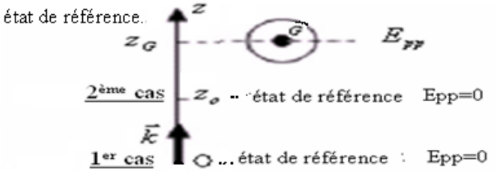
\includegraphics[width=0.5\textwidth]{./img/img00.png}
%\end{wrapfigure}

\section{INTRODUCTION : }

Messagers porteurs, pigeons voyageurs, signaux de fumée, signaux audibles (tam-tam), télégraphe, téléphone,
radio, télévision sans fil, internet... Depuis toujours, l’Homme a cherché à transmettre des messages, le plus vite
et le plus loin possible... Nous étudierons dans ce chapitre comment peuvent être transmises les informations
d’un bout à l’autre du monde ou même dans l’espace, ainsi que la nécessité de coder puis décoder l’information
pour pouvoir la transmettre.
La transmission rapide d’information sans fil est devenue une banalité : sur quel principe repose-t-elle ?
On ne s’intéresse dans ce programme qu’aux transmissions de type radio (sans fil) encore appelées
transmissions hertziennes. Le support est une onde, appelée onde porteuse, sur laquelle, on greffe l’information
à transporter. On dit que l’onde porteuse a été modulée par le signal à transmettre.

\section{Les Ondes électromagnétiques- Transmission d'informations. }



\subsection{Définition : }
Une onde électromagnétique est composée d’un champ électrique et d’un champ magnétique qui se
propagent tous deux à la même vitesse. Dans le vide, les ondes électromagnétiques se propagent à la célérité
de la lumière : $c = 3.10^8 m.s^{-1}$ . 

\begin{center}

  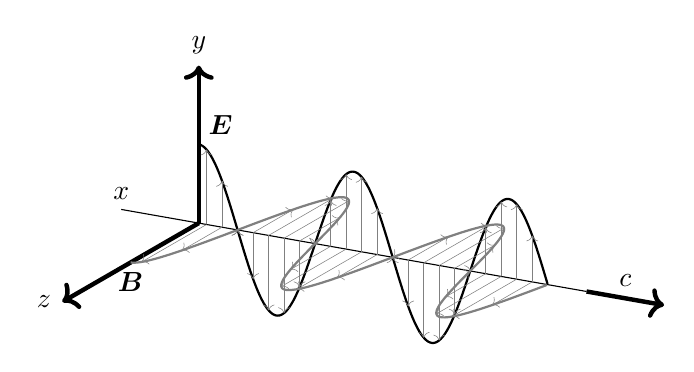
\begin{tikzpicture}[x={(-10:1cm)},y={(90:1cm)},z={(210:1cm)}]
    % Axes
    \draw (-1,0,0) node[above] {$x$} -- (5,0,0);
	\draw[->,ultra thick] (0,0,0) -- (0,2,0) node[above] {$y$};
    \draw [->,ultra thick](0,0,0) -- (0,0,2) node[left] {$z$};
    % Propagation
    \draw[->,ultra thick] (5,0,0) -- node[above] {$c$} (6,0,0);
    % Waves
    \draw[thick] plot[domain=0:4.5,samples=200] (\x,{cos(deg(pi*\x))},0);
    \draw[gray,thick] plot[domain=0:4.5,samples=200] (\x,0,{cos(deg(pi*\x))});
    % Arrows
    \foreach \x in {0.1,0.3,...,4.4} {
      \draw[->,help lines] (\x,0,0) -- (\x,{cos(deg(pi*\x))},0);
      \draw[->,help lines] (\x,0,0) -- (\x,0,{cos(deg(pi*\x))});
    }
    % Labels
    \node[above right] at (0,1,0) {$\bm{E}$};
    \node[below] at (0,0,1) {$\bm{B}$};
  \end{tikzpicture}

\end{center}
Les ondes électromagnétiques n’ont pas besoin de support matériel pour se
propager. On observe des phénomènes de diffraction, d’interférence, elles se réfléchissent et se réfractent
comme les ondes lumineuses ce qui montre que les ondes lumineuses sont des ondes électromagnétiques.
Les ondes hertziennes, utilisés dans le domaine de la radio, la télévision, la téléphonie mobile sont également
des ondes électromagnétiques.

\subsection{ La classification des ondes  électromagnétiques:}
Les ondes hertziennes sont utilisées dans les télécommunications. Leurs domaines de fréquences sont
indiqués par le document suivant :

\begin{center}
	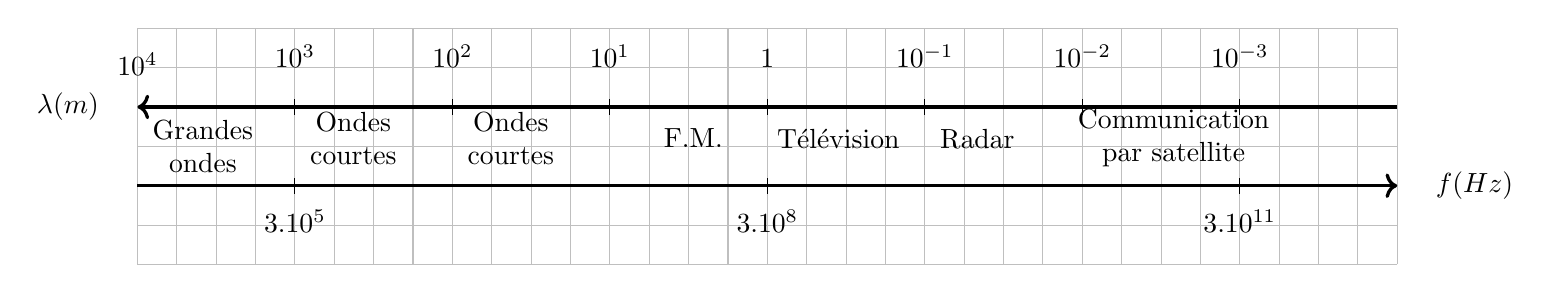
\begin{tikzpicture}

		\draw[step=0.5,lightgray] (0,0) grid (16,3);
		\draw[<-, very thick] (0,2) node[above, left=10pt]{$\lambda(m)$}-- (16,2);

		\coordinate (A) at (0,2);
		\draw (A) node[above, above=8pt]{$10^4$} node[below, below = 0.5cm,right=2,align=center] {Grandes\\ondes};
		\draw (2,1.9)    -- (2,2.1) node[above, above=8pt]{$10^3$}
							node[below, below = 0.5cm,right=2,align=center]{Ondes\\courtes}
			  (4, 1.9) -- (4, 2.1)  node[above, above=8pt]{$10^2$}
							node[below, below = 0.5cm,right=2,align=center]{Ondes\\courtes}
			  (6,1.9) -- (6,2.1)   node[above, above=8pt]{$10^1$}
							node[below, below = 0.5cm,right=16,align=center]{F.M.}
			  (8,1.9) -- (8,2.1)   node[above, above=8pt]{$1$}
							node[below, below = 0.5cm,right=0,align=center]{Télévision}
							(10,1.9) -- (10,2.1)   node[above, above=8pt]{$10^{-1}$}
							node[below, below = 0.5cm,right=2,align=center]{Radar}
							(12,1.9) -- (12,2.1)   node[above, above=8pt]{$10^{-2}$}
							node[below, below = 0.5cm,left=-2.5cm,align=center]{Communication\\par satellite}
							(14,1.9) -- (14,2.1)   node[above, above=8pt]{$10^{-3}$}



			  ;


		\draw[->,very thick] (0,1) -- (16,1) node[above, right=10pt] {$f(Hz)$};

							\draw (14,0.9) -- (14,1.1)   node[below, below=8pt]{$3.10^{11}$};
							\draw (8,0.9) -- (8,1.1)   node[below, below=8pt]{$3.10^{8}$};
							\draw (2,0.9) -- (2,1.1)   node[below, below=8pt]{$3.10^{5}$};
	\end{tikzpicture}



\end{center}

\subsection{Intérêt des ondes électromagnétiques }
Il réside dans leur mode de propagation : rectiligne, avec une vitesse égale à celle de la lumière, pouvant subir
les phénomènes de réflexion et de réfraction. Les ondes hertziennes se propagent dans le vide. Elles traversent
plus ou moins bien les milieux matériels, mais ne se propagent pas à travers les métaux.

Les ondes électromagnétiques ont de nombreuses utilisations pratiques dans la vie quotidienne. Les exemples incluent :
\begin{itemize}
	\item la transmission de la radio et de la télévision,
	\item la communication mobile (téléphone portable, réseau 4G/5G),
	\item la navigation GPS,
	\item la détection des radar,
	\item la cuisson des aliments au micro-ondes,
	\item la thérapie par rayons X,
\item les technologies sans fil telles que le Wi-Fi et le Bluetooth, les technologies de l'énergie solaire,
\item les technologies de l'énergie éolienne,
\item les technologies de l'Internet des objets (IoT).
\item Les ondes électromagnétiques sont également utilisées dans des domaines tels que l'astronomie, la météorologie, la médecine et l'agriculture. En outre, les ondes électromagnétiques sont utilisées dans de nombreux systèmes industriels pour la détection, la communication, la surveillance et la commande à distance.

\end{itemize}
\subsection{Mise en évidence de la présence d'ondes électromagnétiques :}
\begin{wrapfigure}{r}{0.3\textwidth}
	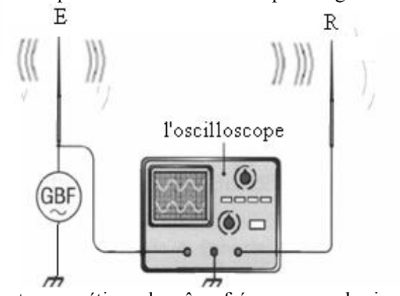
\includegraphics[width=0.3\textwidth]{./img/modulation003.png}
\end{wrapfigure}

Dans le montage suivant E et R sont deux fils électriques conducteurs qui jouent le rôle d'émetteur et de récepteur .
On visualise sur l'entrée $Y_A$ de l'oscilloscope un signal sinusoïdal émis par le générateur GBF et on obtient sur l'entrée YB un
signal reçu par le récepteur R qui la même fréquence et la même forme que le signal émis par E.


L'antenne émettrice E émet une onde électromagnétique de même fréquence que le signal électrique du ciruit .Cette onde se
propage dans tout l'espace et provoque dans l'antenne réceptrice R un signal de même fréquence.
L'onde électromagnétique peut transporter le signal qui contient l'information à des grandes distances sans aucun transport de
la matière et avec une vitesse égale à la célérité de lumière dans le vide.



\subsection{le rôle de la modulation :  }
Pour transmettre un signal de basse fréquence BF à une distance de plusieurs millions de kilomètres, il serait rapidement
atténué et en plus la réception de ce signal nécessitera des antennes de très grandes dimensions, car la longueur de l'antenne est en général de l'ordre de la moitié de la longueur d'onde du signal de réception : $l = \frac{\lambda}{2}$

Pour un signal BF, f=200Hz par exemple, sa longueur d'onde $\lambda = \frac{c}{f} = \frac{3.10^8}{200} = 15.10^5m = 1500km$ , pour le capter on a

besoin d'une antenne de longueur $l = \frac{\lambda}{2} = 750km$

Un signal haute fréquence HF sera facilement transmissible [HF correspond à des fréquences $f> 100MHz$] , de longueurs d'ondes $\lambda = \frac{c}{f}<3m$ et pour le capter l’antenne utilisée sera de longueur inférieure à 1,5m.

Pour cette raison on doit utiliser une technique pour transmettre les informations , cette technique s'appelle la modulation.
La modulation est un processus qui consiste à transmettre le signal de sa forme original en une forme adaptée au canal de
transmission en faisant varier son amplitude ou sa fréquence ou bien sa phase.

\subsection{Les différents types de modulations : }


La technique de modulation consiste à superposer un signal de basse fréquence (le signal modulant) sur un signal de haute fréquence (l'onde porteuse) pour obtenir un signal modulé. Cela permet de transmettre des informations à une fréquence plus élevée, qui peut être plus résistant aux perturbations et parcourir de plus grandes distances. Il existe différents types de modulation, 

\begin{itemize}
	\item tels que la modulation en amplitude (AM), \item la modulation en fréquence (FM) \item  la modulation en phase (PM).
\end{itemize}

\section*{La modulation par amplitude :}
Elle correspond à la modulation de l'amplitude de l'onde porteuse selon le signal modulant contenant l'information. $$u(t) = u_m(t).cos(2\pi.f.t + \phi)$$
\begin{wrapfigure}[1]{r}{10cm}
	%\vspace{cm}
	\begin{center}
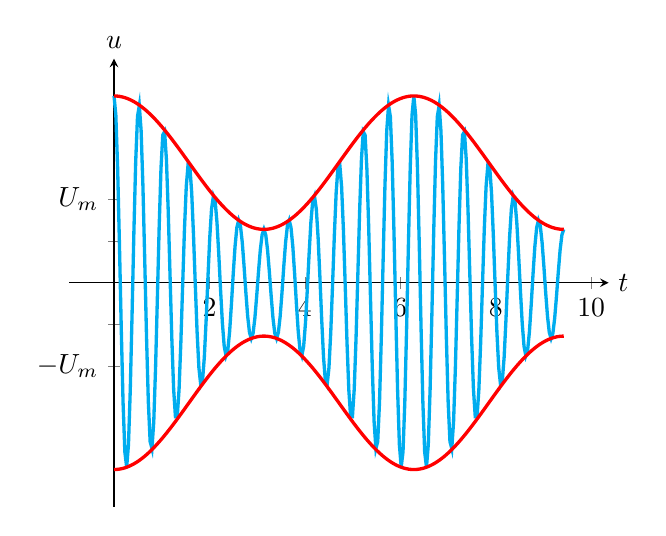
\begin{tikzpicture}
    \begin{axis}[
        trig format plots = rad,
        axis lines = middle,
        enlargelimits,
        xlabel={$t$},
        ylabel={$u$},
        xlabel style={right},
        ylabel style={above},
		%xtick={1,2,3,4,5},
        ytick={1,0.5,-0.5,-1}, 
        yticklabels={$U_m$,,,$-U_m$},
    ]    
    %\addplot[very thick,cyan,domain=0:8*pi,samples=200] {cos(5*deg(x))};

\addplot[very thick,cyan,domain=0:3*pi,samples=250] { (0.8*cos(x) + 1.44)*cos(12*x)};
\addplot[very thick,red,domain=0:3*pi,samples=250] { (0.8*cos(x) + 1.44)};
\addplot[very thick,red,domain=0:3*pi,samples=250] { (-0.8*cos(x) - 1.44)};
    \end{axis}
\end{tikzpicture}
\end{center}
\end{wrapfigure}



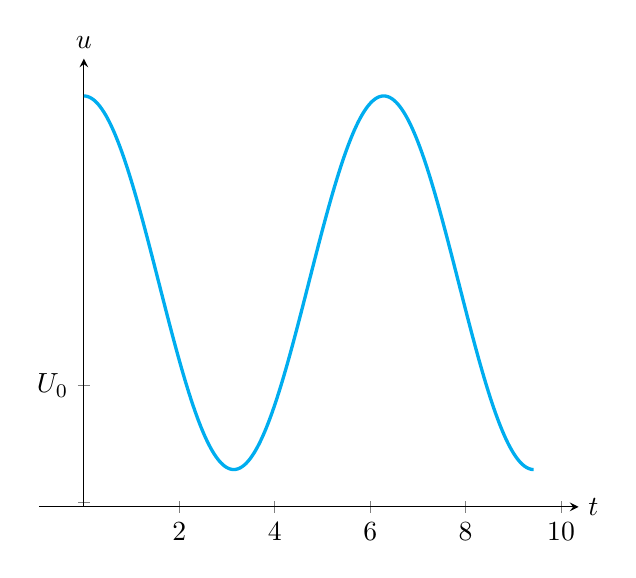
\begin{tikzpicture}
    \begin{axis}[
        trig format plots = rad,
        axis lines = middle,
        enlargelimits,
        xlabel={$t$},
        ylabel={$u$},
        xlabel style={right},
        ylabel style={above},
		%xtick={1,2,3,4,5},
        ytick={1,0.5,-0.5,-1}, 
        yticklabels={$U_0$,,,$-U_m$},
    ]    
\addplot[very thick,cyan,domain=0:3*pi,samples=250] {0.8*cos(x) + 1.44};

    \end{axis}
\end{tikzpicture}



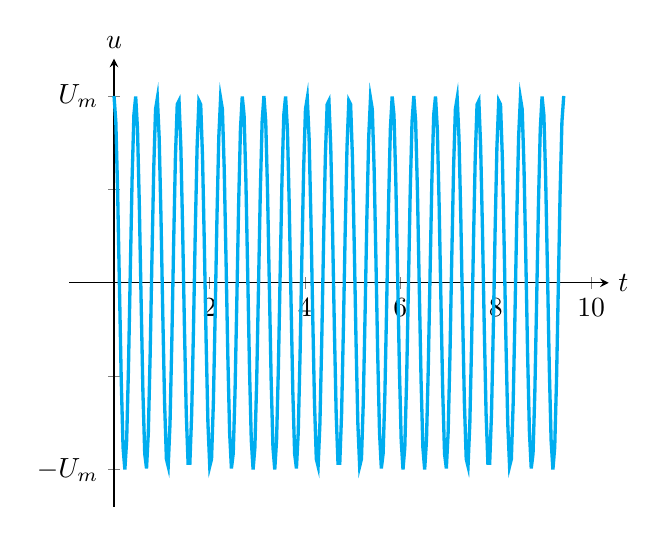
\begin{tikzpicture}
    \begin{axis}[
        trig format plots = rad,
        axis lines = middle,
        enlargelimits,
        xlabel={$t$},
        ylabel={$u$},
        xlabel style={right},
        ylabel style={above},
		%xtick={1,2,3,4,5},
        ytick={1,0.5,-0.5,-1}, 
        yticklabels={$U_m$,,,$-U_m$},
    ]    
    %\addplot[very thick,cyan,domain=0:8*pi,samples=200] {cos(5*deg(x))};

\addplot[very thick,cyan,domain=0:3*pi,samples=250] {cos(14*x)};
    \end{axis}
\end{tikzpicture}



\section*{La modulation de fréquence :}
Elle correspond à une variation de la fréquence de l'onde porteuse par celle de l'information.$$u(t) = u_m.cos(2\pi.f(t).t + \phi)$$
\begin{center}
	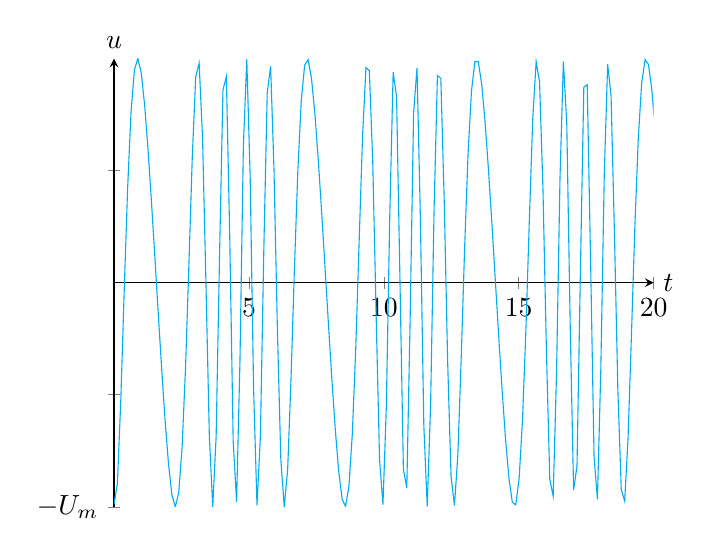
\begin{tikzpicture}
    \begin{axis}[
        trig format plots = rad,
        axis lines = middle,
        %enlargelimits,
        xlabel={$t$},
        ylabel={$u$},
        xlabel style={right},
        ylabel style={above},
        ytick={1,0.5,-0.5,-1}, 
        %xtick={0,...,12}, 
		xmax=20,
        yticklabels={$U_m$,,,$-U_m$},
    ]    
      \addplot[domain=0:10*pi,cyan,samples=250] {cos(5*x + 3*cos(x))};

    \end{axis}
\end{tikzpicture}
\end{center}

\subsection*{La modulation de phase :}
Elle correspond à une variation de la phase de l'onde porteuse par celle de l'information.
$$u(t) = u_m.cos(2\pi.f.t + \phi(t))$$

\section{Modulation d'amplitude:}

\subsection{Définition: }
Le principe de modulation d'amplitude consiste à transmettre une onde de basse fréquence au moyen d'une onde électromagnétique porteuse
de haute fréquence puis par démodulation on obtient le signal transmit.
Parmi les conditions nécessaires pour faire la modulation d'amplitude:
\begin{itemize}
	\item Les signaux basses fréquences sont rapidement amortis avec la distance.
	\item leur vitesse de propagation est faible par rapport à celle des ondes électromagnétiques.
	\item La réception des signaux de basses fréquences nécessitent des antennes de grandes dimensions difficiles à réaliser.
\end{itemize}

\subsection{Le modulateur d'amplitude: }

Le montage expérimental est constitué de deux générateurs GBF plus un oscilloscope et un multiplieur réalisant la modulation.
Le premier générateur GBF fournit un signal s(t) sinusoïdal de basse fréquence décalé :




\begin{itemize}
	\item $s(t)$ le signal sinusoïdal de basse fréquence à transmettre appelé: \underline{\textbf{signal modulant}}, de fréquence $f_s$
	\item Le deuxième générateur GBF fournit un signal $p(t)$ sinusoïdal de haute fréquence (la porteuse), de fréquence $f_p$ très grande par rapport à la fréquence $f_s$.
	\item Pratiquement on utilise un composant électronique AD633 nommé multiplieur symbolisé par X qui multiplie les tensions qui lui sont
appliquées en entrées, et qui donne à sa sortie une tension proportionnelle à ce produit. 

\end{itemize}


\begin{center}
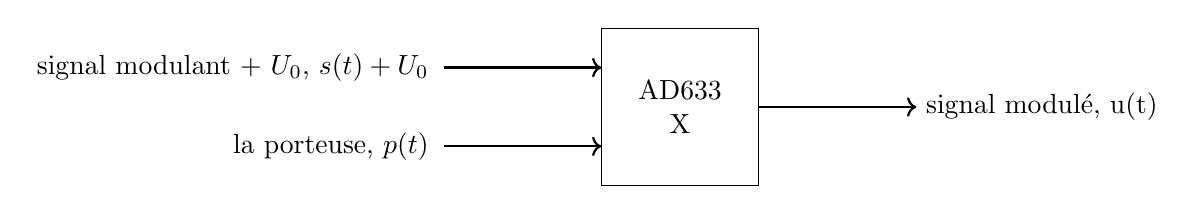
\begin{tikzpicture}
    % Draw the AD633 block
    \draw (1,1) rectangle (3,3);
	\node[align=center] at (2,2) {AD633\\X};
    
    % Draw the input terminals
	\draw[thick,<-] (1,1.5) -- (-1,1.5);
	\draw[thick,<-] (1,2.5) -- (-1,2.5);
	\node at (-1,1.5) [left, left= 2pt] {la porteuse, $p(t)$};
    \node at (-1,2.5) [left, left=2pt] {signal modulant + $U_0$, $s(t)+U_0$};
    
    % Draw the output terminal
	\draw[thick,->] (3,2) -- (5,2);
    \node at (5,2) [right] {signal modulé, u(t)};
    
   \end{tikzpicture}
\end{center}


La tension modulée u(t) obtenue à la sortie du multiplieur est proportionnelle au produit des deux tensions : p(t) et (s(t)+Uo).
s(t) : étant la tension modulante qui représente le signal à transmettre et Uo est une tension constante appelée tension de décalage.

\begin{wrapfigure}[0]{r}{10cm}
	\vspace{-5cm}
	\begin{center}
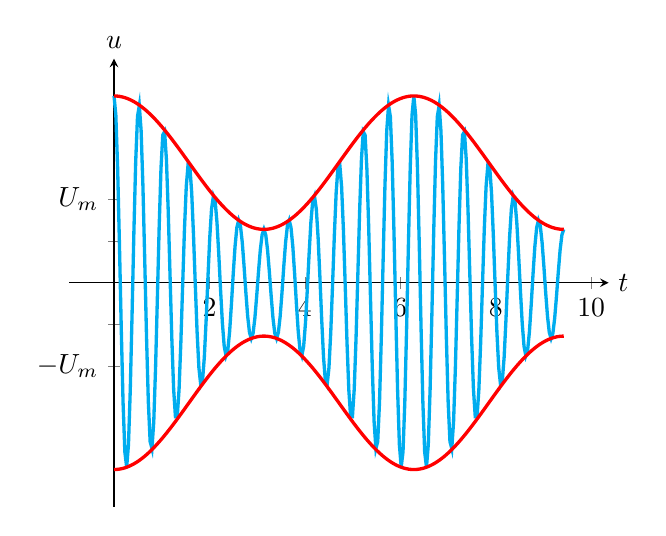
\begin{tikzpicture}
    \begin{axis}[
        trig format plots = rad,
        axis lines = middle,
        enlargelimits,
        xlabel={$t$},
        ylabel={$u$},
        xlabel style={right},
        ylabel style={above},
		%xtick={1,2,3,4,5},
        ytick={1,0.5,-0.5,-1}, 
        yticklabels={$U_m$,,,$-U_m$},
    ]    
    %\addplot[very thick,cyan,domain=0:8*pi,samples=200] {cos(5*deg(x))};

\addplot[very thick,cyan,domain=0:3*pi,samples=250] { (0.8*cos(x) + 1.44)*cos(12*x)};
\addplot[very thick,red,domain=0:3*pi,samples=250] { (0.8*cos(x) + 1.44)};
\addplot[very thick,red,domain=0:3*pi,samples=250] { (-0.8*cos(x) - 1.44)};
    \end{axis}
\end{tikzpicture}

\textbf{La tension modulée $u(t) = K[s(t)+U_0].p(t)$}
\end{center}
\end{wrapfigure}

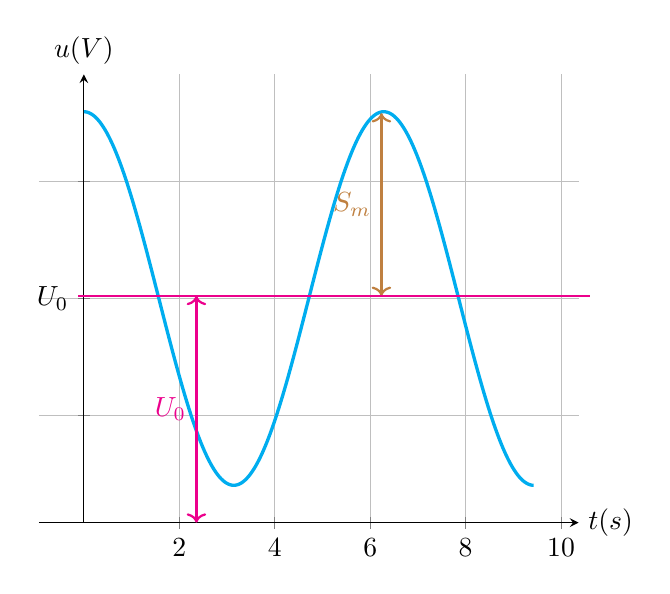
\begin{tikzpicture}
    \begin{axis}[
		    grid,
        trig format plots = rad,
        axis lines = middle,
        enlargelimits,
        xlabel={$t(s)$},
        ylabel={$u(V)$},
        xlabel style={right},
        ylabel style={above},
        ytick={2,1.5,1,0.5,-0.5,-1}, 
        yticklabels={$U_0 + S_m$,,$U_0$,,$-S_m$},
    ]    
\addplot[very thick,cyan,domain=0:3*pi,samples=250] {0.8*cos(x)+1};


    \end{axis}

	\draw[thick,magenta,<->]  (2,0) -- (2,2.88)node [pos=0.5, left] {$U_0$};
	\draw[thick,brown,<->]  (4.35,2.88) -- (4.35,5.2)node [pos=0.5, left] {$S_m$};

	\draw[thick,magenta]  (0.5,2.88) -- (7,2.88);

\end{tikzpicture}

\textbf{signal modulant s(t) + $U_0$ avec $s(t) = S_m.cos(2.\pi.f_s.t)$}

%%%fg                next porteuse


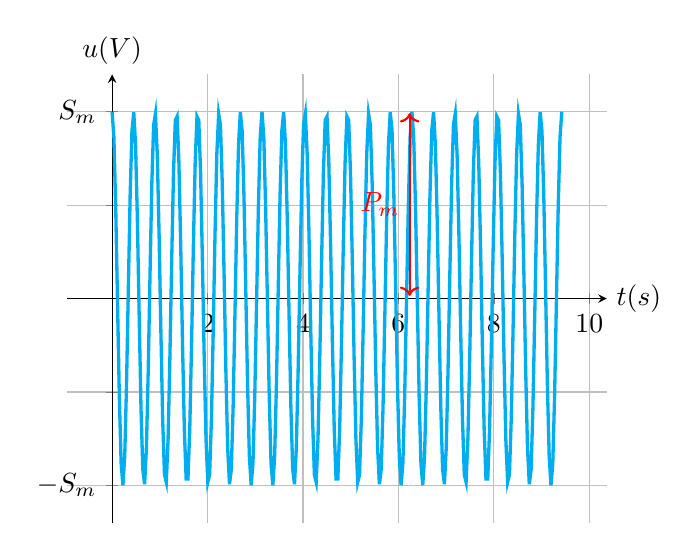
\begin{tikzpicture}
    \begin{axis}[
		    grid,
        trig format plots = rad,
        axis lines = middle,
        enlargelimits,
        xlabel={$t(s)$},
        ylabel={$u(V)$},
        xlabel style={right},
        ylabel style={above},
	ytick={1,0.5,-0.5,-1}, 
        yticklabels={$S_m$,,,$-S_m$},
    ]    
\addplot[very thick,cyan,domain=0:3*pi,samples=250] {cos(14*x)};


    \end{axis}

	%\draw[thick,magenta,<->]  (2,0) -- (2,2.88)node [pos=0.5, left] {$U_0$};
	\draw[thick,red,<->]  (4.35,2.88) -- (4.35,5.2)node [pos=0.5, left] {$P_m$};

	%\draw[thick,magenta]  (0.5,2.88) -- (7,2.88);

\end{tikzpicture}

\textbf{la porteuse p(t) avec $p(t) = P_m.cos(2.\pi.f_p.t)$}

\subsection{Expression de l'amplitude de la tension modulée:}

L'amplitude de la tension modulée (AM) peut être exprimée en fonction des tensions d'amplitude modulante (s(t)) et de porteuse (p(t)) de la manière suivante :

$$u(t) =  k.[s(t)+U_0].p(t)$$
donc $$u(t) = k.[S_m.cos(2\pi.f_s.t)+U_0]P_m.cos(2\pi.f_p.t)$$
alors $$u(t) = K.P_m.U_0[\frac{S_m}{U_0}.cos(2.\pi.f_s.t) + 1].cos(2\pi.f_p.t)$$
On écrit généralement : $$u(t) = A[m.cos(2.\pi.f_s.t) + 1].cos(2\pi.f_p.t)$$
en posant : $A = K.P_m.U_0$ et $m = \frac{S_m}{U_0}$ taux de modulation

On développe $$u(t) = A.m.cos(2.\pi.f_s.t).cos(2\pi.f_p.t) + A.cos(2\pi.f_p.t) $$
Rappel : $cos(a).cos(b) = \frac{1}{2}.cos(a+b) + cos(a-b)$


On écrit  : $$u(t) = A.m.\frac{1}{2}.[cos(2.\pi.(f_s + f_p).t) + cos(2.\pi.(f_s - f_p).t)]  + A.cos(2\pi.f_p.t) $$

On obtient bien une tension u(t), somme de trois fonctions sinusoidales de fréquences: $f_p$, $f_p + f_s$ , $f_p-f_s$

\begin{center}
\begin{tikzpicture}

% axes
\draw[->] (-1,0) -- (5,0) node[right] {$f$};
\draw[->] (0,-1) -- (0,3) node[above] {$A$};

% carrier wave
\draw[cyan] (2,0) -- (2,2);

% modulating wave
\draw[red] (1,0) -- (1,1);
\draw[magenta] (3,0) -- (3,1);
% sidebands
%\draw[magenta] (-0.5,0.5) -- (2.5,0.5);
%\draw[magenta] (-0.5,1.5) -- (2.5,1.5);

% labels
\node at (0,1) [left] {$\frac{A.m}{2}$};
\draw[dashed] (0,2)node[left] {A} -- (2,2);
\draw[dashed] (0,1) -- (3,1);
\node at (1,0) [below] {$f_p - f_s$};
\node at (2,0) [below] {$f_p$};
\node at (3,0) [below] {$f_p + f_s$};

\end{tikzpicture}
\end{center}


De la relation ci-dessous , montre que l’amplitude modulée Um(t) varie
entre deux valeurs extrêmes $Um_{min}$ et $Um_{max}$
tel que :  $Um_{max} = A(m+1)$ et   $Um_{min} = A(-m+1)$

c’est à dire que :$Um_{max} + Um_{min} = 2A.m$  ET $Um_{max} - Um_{min} = 2A$

d’où le taux de modulation est :$$m = \frac{Um_{max } - Um_{min}}{Um_{max} + Um_{min}}$$

\begin{itemize}
	\item L'enveloppe du signal modulé a la même forme et la même fréquence que le signal modulant.
	\item L'amplitude du signal modulé varie entre deux valeurs $Um_{max}$ et $Um_{min}$.
	\item La modulation est bonne qualité si l'enveloppe du signal modulé correspond au signal modulant.
\end{itemize}

\subsection{Qualité de modulation : }

\section*{1-Premier cas : $m < 1$}
On constate que la tension modulée u(t) a une enveloppe qui correspond
parfaitement au signal modulant s(t) .
La modulation dans ce cas est de bonne qualité.


Pour s’assurer que la modulation est de bonne qualité on utilise la
méthode du trapèze qui représente us(t) en fonction de s(t) .
Pratiquement on suit la démarche suivante :

\begin{itemize}
	\item La grande base représente $2Um_{max}$
	\item la petite base représente $2Um_{min}$
	\item la relation entre le taux demodulation et  les dimensions du trapèze : $m = \frac{B-b}{B+b}$

	\item $Um_{max}$ :amplitude maximale du signal modulé
	\item $Um_{min}$:Tamplitude minimale du signal modulé.
\end{itemize}

	\begin{center}
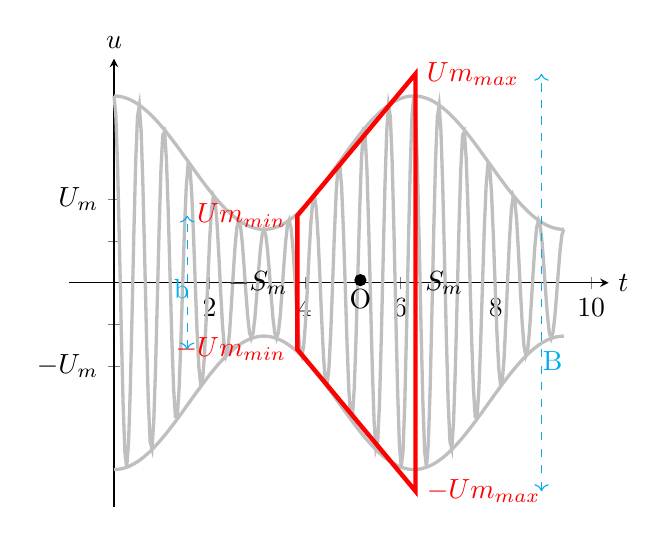
\begin{tikzpicture}
    \begin{axis}[
        trig format plots = rad,
        axis lines = middle,
        enlargelimits,
        xlabel={$t$},
        ylabel={$u$},
        xlabel style={right},
        ylabel style={above},
		%xtick={1,2,3,4,5},
        ytick={1,0.5,-0.5,-1}, 
        yticklabels={$U_m$,,,$-U_m$},
    ]    
    %\addplot[very thick,cyan,domain=0:8*pi,samples=200] {cos(5*deg(x))};

\addplot[very thick,lightgray,domain=0:3*pi,samples=250] { (0.8*cos(x) + 1.44)*cos(12*x)};
\addplot[very thick,lightgray,domain=0:3*pi,samples=250] { (0.8*cos(x) + 1.44)};
\addplot[very thick,lightgray,domain=0:3*pi,samples=250] { (-0.8*cos(x) - 1.44)};
    \end{axis}

% define coordinates
	\coordinate (A) at (2.9,2);
	\coordinate (B) at (4.4,0.2);
\coordinate (C) at (2.9,3.7);
\coordinate (D) at (4.4,5.5);

% draw trapezoid
%\draw[ultra  thick,black] (A) node[below]{A} -- (B) node[below] {B};
%\draw[ultra thick,black] (C) node[above]{C} -- (D) node[above] {D};

\draw[ultra thick,red] (A) node[left]{$-Um_{min}$}-- (B) node[right]{$-Um_{max}$}-- (D) node[right]{$Um_{max}$}-- (C)node[left]{$Um_{min}$}--cycle;
\draw (4.4, 2.84) node[right] {$S_m$};
\draw (2.9, 2.84) node[left] {$-S_m$};

\draw[dashed, <->,cyan] (6,0.2) node[right=4pt,above=40pt]{B} -- (6,5.5);
\draw[dashed, <->,cyan] (1.5,2) node[left = 2pt, above=15pt]{b} -- (1.5,3.7);

\filldraw[black] (3.7,2.88) node[below] {O} circle (2pt);

\end{tikzpicture}

\textbf{La tension modulée $u(t) = K[s(t)+U_0].p(t)$}
\end{center}




\section*{2-Premier cas : $m > 1$}

On constate que la tension modulée us(t) possède une enveloppe qui
n’est pas semblable à la tension modulante s(t) . La modulation dans
ce cas est mauvaise qualité
ce phénomène s’appelle sur-modulation.
	\begin{center}
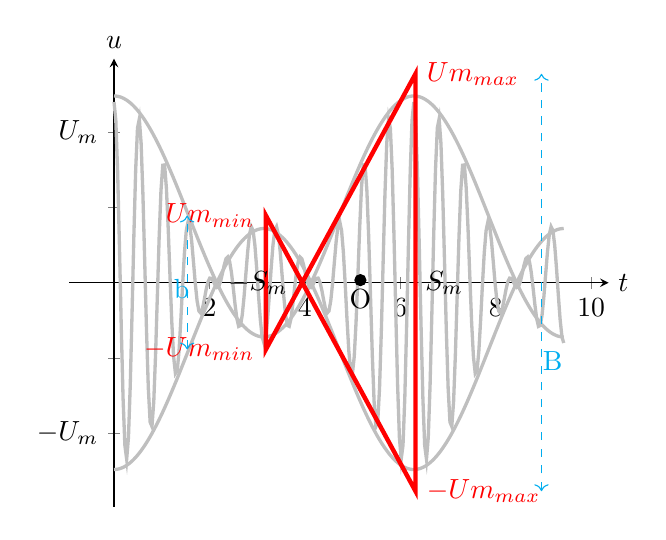
\begin{tikzpicture}
    \begin{axis}[
        trig format plots = rad,
        axis lines = middle,
        enlargelimits,
        xlabel={$t$},
        ylabel={$u$},
        xlabel style={right},
        ylabel style={above},
		%xtick={1,2,3,4,5},
        ytick={1,0.5,-0.5,-1}, 
        yticklabels={$U_m$,,,$-U_m$},
    ]    
    %\addplot[very thick,cyan,domain=0:8*pi,samples=200] {cos(5*deg(x))};

\addplot[very thick,lightgray,domain=0:3*pi,samples=250] { (0.8*cos(x) + 0.4)*cos(12*x)};
\addplot[very thick,lightgray,domain=0:3*pi,samples=250] { (0.8*cos(x) + 0.44)};
\addplot[very thick,lightgray,domain=0:3*pi,samples=250] { (-0.8*cos(x) - 0.44)};
    \end{axis}

% define coordinates
	\coordinate (A) at (2.5,2);
	\coordinate (B) at (4.4,0.2);
\coordinate (C) at (2.5,3.7);
\coordinate (D) at (4.4,5.5);

% draw trapezoid
%\draw[ultra  thick,black] (A) node[below]{A} -- (B) node[below] {B};
%\draw[ultra thick,black] (C) node[above]{C} -- (D) node[above] {D};

\draw[ultra thick,red] (A) node[left]{$-Um_{min}$}--  (D) node[right]{$Um_{max}$}-- (B) node[right]{$-Um_{max}$}--(C)node[left]{$Um_{min}$}--cycle;
\draw (4.4, 2.84) node[right] {$S_m$};
\draw (2.9, 2.84) node[left] {$-S_m$};

\draw[dashed, <->,cyan] (6,0.2) node[right=4pt,above=40pt]{B} -- (6,5.5);
\draw[dashed, <->,cyan] (1.5,2) node[left = 2pt, above=15pt]{b} -- (1.5,3.7);

\filldraw[black] (3.7,2.88) node[below] {O} circle (2pt);

\end{tikzpicture}

\textbf{La tension modulée $u(t) = K[s(t)+U_0].p(t)$}
\end{center}

Quand la modulation est mauvaise qualité, l'enveloppe du signal modulé n'est pas identique au signal modulant .Cela est dû au fait que le
décalage en tension Uo est inférieur à l'amplitude Sm du signal modulant, $m=\frac{S_m}{U_0}>1$ soit $U_0 < S_m$ on dit qu’il y'a surmodulation.

\textbf{Pour éviter la surmodulation} le décalage Uo doit être supérieur à Sm ce qui permet par la suite la restitution du signal initial complet par
démodulation.

\begin{tcolorbox}
Conditions d’obtention d’une bonne modulation
Pour obtenir une modulation d’amplitude de bonne qualité il faut que :
\begin{itemize}
	\item  La tension de décalage U0 doit être plus grande à l’amplitude Smde la
tension modulante : $U0 > Sm$ i.e que $m < 1$
\item La fréquence Fp de la tension porteuse doit être supérieure à la
fréquence fS de la tension modulante. $(Fp >> fs)$. Au minimum
$Fp > 10.fs$

\end{itemize}
\end{tcolorbox}


\section{La démodulation:}
\subsection{Définition:}
La démodulation consiste à récupérer au niveau du récepteur le signal modulant qui contient l'information et qui représente la partie
supérieure du signal modulé. Elle s'opère en deux étapes:

- La détection d'enveloppe.

- L'élimination de la tension continue par filtrage.

\subsection{Les étapes de démodulation: }
\section*{1ère étape: }

Suppression des alternances négatives et élimination de l’enveloppe.
Le montage utilisé est un filtre passe-bas qui comporte une diode qui bloque les alternances négatives et on obtient une tension redressée.
\begin{center}
    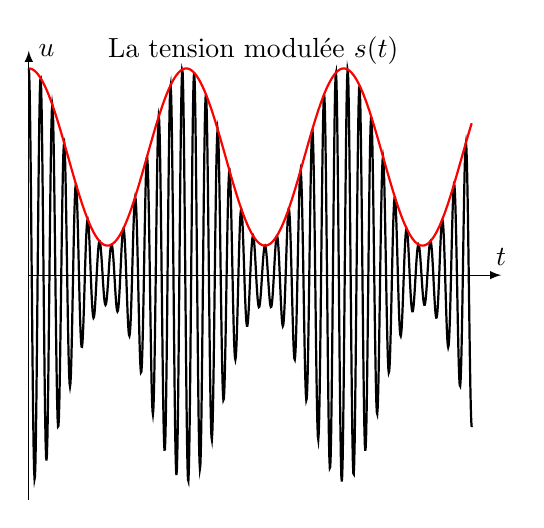
\begin{tikzpicture}[scale=0.75]
\draw[-latex, smooth] (0,0)--(8,0) node[above] {$t$};
\draw[-latex, smooth] (0,-3.8)--(0,3.8) node[right] {$u$};
\draw[thick] plot[domain=0:7.5,samples=1000] (\x,{cos(10*pi*\x r)*(1.5*cos(0.75*pi*\x r)+2)});
\draw[thick,red] plot[domain=0:7.5,samples=1000] (\x,{(1.5*cos(0.75*pi*\x r)+2)});
\node at (3.8,3.8) {La tension modulée $s(t)$};
\end{tikzpicture}

   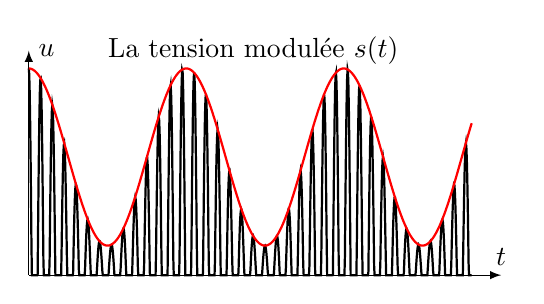
\begin{tikzpicture}[scale=0.75]
\draw[-latex, smooth] (0,0)--(8,0) node[above] {$t$};
\draw[-latex, smooth] (0,0)--(0,3.8) node[right] {$u$};
\draw[thick] plot[domain=0:7.5,samples=1000] (\x,{max(0,cos(10*pi*\x r)*(1.5*cos(0.75*pi*\x r)+2))});

\draw[thick,red] plot[domain=0:7.5,samples=1000] (\x,{(1.5*cos(0.75*pi*\x r)+2)});
\node at (3.8,3.8) {La tension modulée $s(t)$};
    \end{tikzpicture}
\end{center}
	En associant la diode et le filtre passe-bas (qui élimine la partie restante de la porteuse) on obtient le détecteur d’enveloppe .

\begin{circuitikz}[scale=1,transform shape]
            \draw
            %(0,1) node [] {} to [R, l=$R_t$, i>^=$I_t$] (2,1)
            %(0,1) to [cspst=$u$] (1.5,1)
			(3.5,-1) node [] {} -- (6,-1)
            %(0,-1) {to [battery, l_=$V_s$] (0,1)}
            %(1.5,1) to [L, l=$L_1$, i>^=$I_1$] (1.5,-1)
            %(1.5,1) to [C, l=$C_1$, v<={{$V_1$}}] (3.5,1)
			%(3.5,1) {to [diode] (3.5,-1)}
            (3.5,1) to [diode] (5,1)
            (5,1) to [C, l_=$C_1$, ] (5,-1)
            (6,-1) {to [R, l_=$R1$] (6,1)}
            (5,1) -- (6,1);

        \end{circuitikz}
   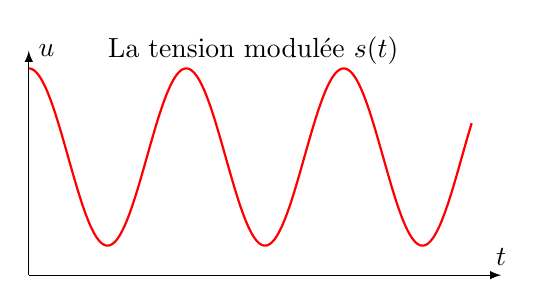
\begin{tikzpicture}[scale=0.75]
\draw[-latex, smooth] (0,0)--(8,0) node[above] {$t$};
\draw[-latex, smooth] (0,0)--(0,3.8) node[right] {$u$};

\draw[thick,red] plot[domain=0:7.5,samples=1000] (\x,{(1.5*cos(0.75*pi*\x r)+2)});
\node at (3.8,3.8) {La tension modulée $s(t)$};
    \end{tikzpicture}

	\begin{tcolorbox}
	Remarque: Pour obtenir une bonne détection d'enveloppe il faut que la constante de temps du dipôle $R_1C_1$ vérifie la condition suivante:
	\begin{itemize}
		\item $T_p<< \tau < T_s$
		\item bonne détection d'enveloppe $T_p<< R_1.C_1 < T_s$ donc $f_s<< \frac{1}{R_1C_1} < f_p$
	\end{itemize}
\end{tcolorbox}

\section*{2.ème étape:}

Elimination de la tension constante de décalage Uo. Cette dernière étape consiste à éliminer la tension constante pour cela on utilise un filtre passe-haut.
Le condensateur C2 élimine la tension Uo et on obtient le montage final de démodulation.



\begin{circuitikz}[scale=1,transform shape]
            \draw
            %(0,1) node [] {} to [R, l=$R_t$, i>^=$I_t$] (2,1)
            %(0,1) to [cspst=$u$] (1.5,1)
			(3.5,-1) node [] {} -- (6,-1)
            %(0,-1) {to [battery, l_=$V_s$] (0,1)}
            %(1.5,1) to [L, l=$L_1$, i>^=$I_1$] (1.5,-1)
            %(1.5,1) to [C, l=$C_1$, v<={{$V_1$}}] (3.5,1)
			%(3.5,1) {to [diode] (3.5,-1)}
            (3.5,1) to [diode] (5,1)
            (5,1) to [C, l_=$C_1$, ] (5,-1)
            (6,-1) {to [R, l_=$R_1$] (6,1)}
            (5,1) -- (6,1);
			\draw 
			(6,1) --(8,1) to [C,l_=$C_2$] (10,1) to [R,l_=$R_2$] (10, -1) -- (3.5,-1);

			\draw[very thick,dashed,cyan] (3,-1.3)node[below,align=center] {détecteur\\d'enveloppe} rectangle (7,1.3);
			
			\draw[very thick,dashed,brown] (8,-1.3)node[below,align=center] {Elimination de la tension\\Constante de décalage} rectangle (11,1.3);
        \end{circuitikz}

		\section{Réalisation d’un dispositif permettant de capter une émission radio
en modulation d’amplitude:}

Un récepteur radio AM se compose les éléments suivants:
\begin{itemize}
	\item Une antenne qui capte les ondes radio.
	\item Un circuit LC pour sélectionner la fréquence de l'onde porteuse que l'on veut capter.

	\item	Cette sélection se réalise en faisant varier l'inductance de la bobine ou la capacité du condensateur jusqu'à ce la fréquence propre fo du
circuit LC soit égale à la fréquence de l'onde porteuse $f_0 = f_p$

avec $$f_0 = \frac{1}{2\pi\sqrt{LC}}$$
La fréquence propre fo du circuit LC :

\item On utilise un amplificateur après la réception et après la modulation du signal modulé.

\item Un circuit de démodulation d'amplitude qui comporte un circuit de détection d'enveloppe et un autre d'élimination de la tension constante.
\end{itemize}


\begin{center}
	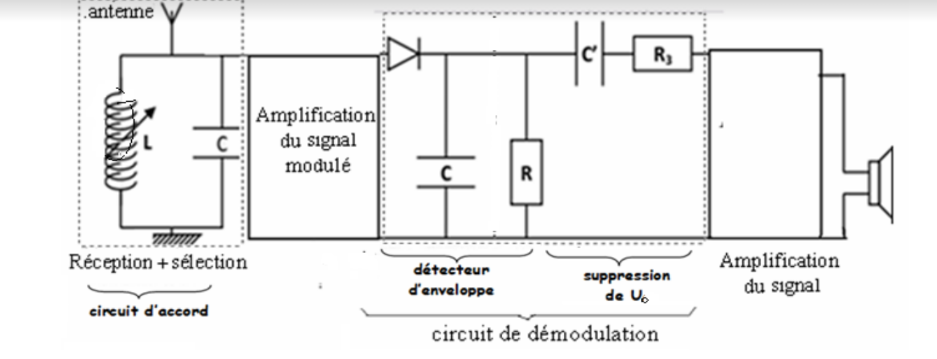
\includegraphics[width=1\textwidth]{./img/mod.png}
\end{center}


%wfg---------------------------------------------------------------sf 
%\begin{center}
   %\begin{tabular}{ |c|c|c|c|c|c|c| }
      %\hline
      %km & hm & dam & \bf{m} & dm & cm & mm \\
      %\hline
        %&   &    &  &   &   & \\
%\hline
%\end{tabular}
%On place un seul nombre dans chaque case.
%\end{center}
%\begin{center}
   %\begin{tabular}{ |c|c|c|c|c|c|c| }
      %\hline
      %$km^2$ & $hm^2$ & $dam^2$ & \bf{$m^2$} & $dm^2$ & $cm^2$ & $mm^2$ \\
      %\hline
        %&   &    &  &   &   & \\
%\hline
%\end{tabular}
%\end{center}


\end{document}

